\documentclass[border=10pt]{standalone}
\usepackage{tikz}
\usetikzlibrary{arrows.meta, positioning}

\begin{document}
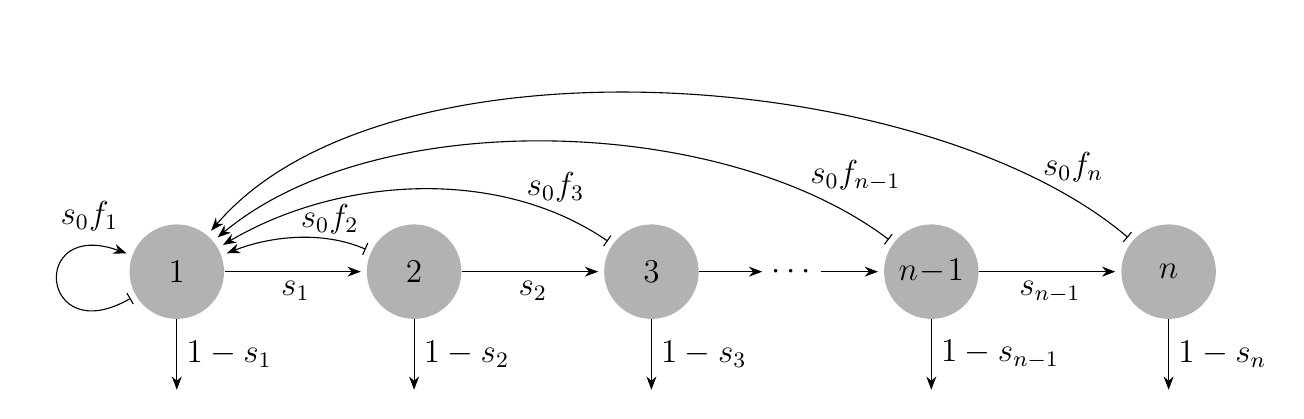
\begin{tikzpicture}[state/.style={circle, draw=none, fill=gray!60, inner sep=0pt, minimum size=1.2cm}, every node/.style={font=\large}, >=Stealth]
	% Nodes
	\node[state] (1) {1};
	\node[state, right=1.8cm of 1] (2) {2};
	\node[state, right=1.8cm of 2] (3) {3};
	\node[right=0.8cm of 3] (dots) {$\cdots$};
	\node[state, right=0.8cm of dots] (n1) {$n\!-\!1$};
	\node[state, right=1.8cm of n1] (n) {$n$};

	% Down arrows and labels
	\draw[->] (1) -- ++(0,-1.5) node[midway, right] {$1 - s_1$};
	\draw[->] (2) -- ++(0,-1.5) node[midway, right] {$1 - s_2$};
	\draw[->] (3) -- ++(0,-1.5) node[midway, right] {$1 - s_3$};
	\draw[->] (n1) -- ++(0,-1.5) node[midway, right] {$1 - s_{n-1}$};
	\draw[->] (n) -- ++(0,-1.5) node[midway, right] {$1 - s_n$};

	% Forward transitions
	\draw[->, shorten >=2pt] (1) -- (2) node[midway, below] {$s_1$};
	\draw[->, shorten >=2pt] (2) -- (3) node[midway, below] {$s_2$};
	\draw[->] (3) -- (dots) node[midway, below] {};
	\draw[->, shorten >=2pt] (dots) -- (n1) node[midway, below] {};
	\draw[->, shorten >=2pt] (n1) -- (n) node[midway, below] {$s_{n-1}$};

	% Backward transitions from 0
	\draw[|->, bend right=25, looseness=0.9, shorten >=2pt, shorten <=2pt, in=200] (2) to node[above, xshift=12pt, yshift=-2pt] {$s_0 f_2$} (1);
	\draw[|->, bend right=35, looseness=0.9, shorten >=2pt, shorten <=2pt, in=210] (3) to node[above, xshift=50pt, yshift=-8pt] {$s_0 f_3$} (1);
	\draw[|->, bend right=37, looseness=0.8, shorten >=2pt, shorten <=2pt, in=220] (n1) to node[above, xshift=110pt, yshift=-21pt] {$s_0 f_{n-1}$} (1);
	\draw[|->, bend right=40, looseness=0.75, shorten >=2pt, shorten <=2pt, in=230] (n) to node[above, xshift=150pt, yshift=-35pt] {$s_0 f_n$} (1);

	% Self loop
	\draw[|->, looseness=7, out=210, in=160, shorten >=2pt, shorten <=2pt] (1) to node[above, xshift=11pt, yshift=15pt] {$s_0 f_1$} (1);
\end{tikzpicture}
\end{document}
